\documentclass{jsarticle}
\renewcommand{\figurename}{Figure }
\renewcommand{\tablename}{Table }
\renewcommand{\refname}{References}
\usepackage{multicol, comment, amsmath,endnotes}
\usepackage[dvipdfmx]{graphicx}
\usepackage[hypertex]{hyperref}
\usepackage{endnotes}
\let\footnote=\endnote
\renewcommand{\theendnote}{\roman{endnote})}
\usepackage{etoolbox}
\patchcmd{\enoteformat}{1.8em}{0pt}{}{}

\pagestyle{myheadings}

\makeatletter
\newenvironment{tablehere}
  {\def\@captype{table}}
  {}
\newenvironment{figurehere}
  {\def\@captype{figure}}
  {}
\makeatother

\setlength{\abovedisplayskip}{20pt}
\setlength{\belowdisplayskip}{20pt}

\begin{document}

\title{Dynamics of Cumulative Culture with Microfoundation}
\author{49-167101 Kensuke Ito\footnote{A doctoral student of Graduate School of Interdisciplinary Information Studies in The University of Tokyo \newline Keywords: {\sl cultural evolution, cumulative culture, economic growth theory}}}
\date{}
\maketitle

\begin{comment}
    \section*{Abstract}
    本研究の目的は、文化が累積的に進化する過程を、同様に人間の活動の結果として生じる蓄積を取り扱う経済成長理論の手法を用いて表現することである。
    作成したモデルからは、以下2点の主要な結論が導かれた。
    第一に、文化ストック量の定常解はその質と評価率の影響を受けない。
    第二に、この定常解は考えられる全ての経路に対してほば安定的である。
    これらの結果は、知識の取得費用や減耗、個人の創造性に介入する間接的な文化政策にこそ本質的な効果があることを示唆している。

    This paper presents a dynamics of cumulative culture by using the methodology of economic growth theory which similarly deals with the accumulation stemming from human activities.
    Two main results can be derived from the model we set.
    First, the steady-state value of cultural stock is not affected by its quality and evaluation.
    Second, the steady-state is almost stable in all transitional dynamics.
    These imply that only indirect intervention has the real effect on cultural stock which is especially related to acquisition cost, depreciation and creativity.
\end{comment}

\section{Introduction}

Theories on cumulative culture have been developed mainly in the field of cultural evolution which is an application of darwinian evolutionary process to cultural phenomena.
To find the reason why only human-beings appear to achieve high cultural complexity,
they have not simply quoted the concepts of preceding studies represented by \hyperlink{boyd}{Boyd and Richerson(1985)}
but focused on several aspects which might be related to the accumulation of cultural traits.
For example, \hyperlink{henrich}{Henrich(2004)} presented the contribution of population size to cumulative culture;
\hyperlink{mesoa}{Mesoudi(2011a)} clarified the restriction caused by the acquisition cost of accumulated knowledge;
\hyperlink{lehman}{Lehman et al.(2013)} calculated the optimal strategy of time allocation for learning schedules.

The aim of this study is to add a different dynamics by using the methodology of economic growth theory which values rationality and expectation of individuals.
In general, economics in the mainstream has been considered to be different from cultural evolution in terms of both concepts and methods\footnote{See \hyperlink{mesob}{Mesoudi(2011b), p.21. and pp.177-188.}, for example.}.
However, if we focus on the {\sl cumulative} aspects, there are actually several similarities including the following two points.
First, both deal with the macro-scale dynamics resulting from the accumulation of some micro-scale activities.
Economics has also provided various microfounded dynamic models for capital accumulation, whereas static aspects are often emphasized by cultural evolutionists.
Second, both have a strong tendency of prediction or purpose-orientation.
Although the tendency has been treated carefully in cultural evolution as ``guided variation",
cumulative culture is especially the field where it contains since cultural accumulation is almost peculiar to human-beings who seem to be more rational than other species.
Therefore, we can say that it is worth applying the methodology of economic growth theory to cumulative cultural evolution.

This paper is composed of five chapters including this introduction. Chapter 2 provides an explanation of the structure of our model. Chapter 3 deals with the derivation of its steady-state with several interpretations. Then, Chapter 4 covers the confirmation of its stability by means of phase diagrams. Finally, Chapter 5 summarizes implication and conclusion.

\section{Model}

To emphasize the role of rationality and expectation, our model is constructed of two main components: cultural stock and individuals seeking to maximize their utility.

Cultural stock is the state variable which denotes the amount of accumulated knowledge in a society\footnote{Specifically, this means the sum of all information stored in goods or individuals which corresponds to the term ``genotype" in biology. Because of the difficulty of its quantification, however, most empirical studies analyze cultural ``phenotype" which is the observable characteristics as a result of background information such as shape, color and motion.}.
Note that it is assumed to be homogeneous for simplification; in other words, the effect of cultural diversity is eliminated here.
Individuals, on the other hand, have the role of amplifying cultural stock in each period by using existing stock and their effort as the control variable.
In addition, there is no-human capital and no-uncertainty; that is, individuals can precisely predict the amount of cumulative culture even though they cannot memorize what they have learned.

Specifically, their reproduction is according to the following Cobb-Dougras function\footnote{Linearity in $h_{t}$ is just for the simplification. We can derive the same main conclusions by using more generalized forms including Cobb-Douglas and even CES production function.},
\begin{eqnarray} % production function
    Y_{t} =
    Y(K_{t}, h_{t}) =
    K_{t}^\alpha h_{t}
\end{eqnarray}

\noindent where $Y_{t}$ is the reproduced culture at time  $t$,
$K_{t}$ is cultural stock, and $h_{t}$ is the amount of effort allocated for reproduction.
While it is called capital share in economics, we here define $\alpha$ as the parameter of cultural quality: how existing culture can contribute to reproduction.
This is an analogy of the case that academic papers are often evaluated by the number of citations.
Therefore, the function intuitively means the process by which individuals make new culture by mixing existing culture and their effort just like researchers write new papers by referring to previous studies.

It is important to note that we do not impose any constraints on $\alpha$.
In addition to ordinary increasing function, for the model deals with culture, $Y_{t}$ can be a decreasing function with respect to $K_{t}$
if we assume the easiest culture is likely to be made first and cultural accumulation gradually lessens the room for future reproduction\footnote{\hyperlink{romer}{Romer(2011), pp.103-104.} assumes the same condition in the field of R\&D.}\footnote{Hence, $|\alpha|$ would be more accurate for the parameter of quality rather than $\alpha$.}. Therefore, we consider $\alpha$ to be both positive and negative.
This assumption allows for richer transitional dynamics which we shall confirm later.

Then, only the fraction of $Y_{t}$ is assumed to be evaluated and inherited to the future as flow\footnote{\hyperlink{csik}{Csikszentmihalyi(2014)} proposes similar framework from a viewpoint of creativity named {\sl systems model}.},
\begin{eqnarray} % evaluated culture
    M_{t} =
    M(K_{t}, h_{t}) =
    pY_{t} =
    pK_{t}^\alpha h_{t}
\end{eqnarray}

\noindent where the amount of cultural flow is represented by $M_{t}$, and $p$ is the exogenous variable for its probability, $0<p<1$.
Although exogenous probability is a strong simplification, it does not affect the main implications of the model.

Finally, we can set the following differential equation for the cultural stock\footnote{Equation (3) has non-constant solutions for any $\alpha \neq 0$.},
\begin{eqnarray} % difference equation for the cultural stock
    \dot{K} =
    M(K_{t}, h_{t}) - \delta K_{t}
\end{eqnarray}

\noindent where $\delta K_{t}$ denotes depreciation and $0<\delta<1$.
In the cumulative culture, obsolescence of previous knowledge or physical depreciation of storage media would be practical examples.

In addition to the dynamics of state variable, objective function needs to be defined for microfoundation.
We assume it is composed of two functions;
$u_{1}$: positive utility through evaluation and $u_{2}$: negative utility through acquisition cost of cultural stock.
If individuals wish to maximize their utility over an infinite horizon, therefore, objective function can be set as follows:
\begin{eqnarray} % objective function
    U =
    \int_{t=0}^{\infty} e^{-\rho t} [u_{1}(M(K_{t}, h_{t})) - u_{2}(K_{t})]dt
\end{eqnarray}

\noindent where $\rho$ is time preference and $\rho > 0$.
Specifically, let $u_{1}$ and $u_{2}$ be CRRA and linear, respectively.
\begin{eqnarray} % utility functions
    u_{1} =
    \frac{M_{t}^{1 - \frac{1}{\sigma}} - 1}{1 - \frac{1}{\sigma}},\:
    u_{2} =
    \eta K_{t}
\end{eqnarray}

\noindent $\sigma$ is the elasticity of intertemporal substitution and $\sigma > 0$,
$\eta $ is the acquisition cost per a unit of culture and $\eta > 0$.
Since the curvature of $u_{1}$ increases as $\sigma$ approaches zero,
we can also interpret $\sigma$ as the parameter of creativity: how much incentive do individuals have for cultural reproduction\footnote{Concretely, $u_{1}$ becomes logarithmic when $\sigma$ equals one and approaches linear as $\sigma$ increases.}.

That is all of the assumptions.
Individuals in the model reproduce new culture by using existing cultural stock and their effort for the utility stemming from its evaluation.
However, on the other hand, they have to decide the optimal amount of effort due to the acquisition cost which increases proportionately to cultural stock.
Particularly in a model with no-human capital, dynamic optimization problem clearly appears since current evaluation leads to increasing future acquisition cost. Thus, we can say that their learning schedule is based on a preference for ``evaluated smoothing" under the constraint of acquisition cost.


\section{Steady State}

According to the above settings, the dynamic optimization problem is given by
\footnote{The transversality condition is not required here since individuals get utility from the evaluation which corresponds not to consumption but to savings in macroeconomic models.},
\begin{eqnarray} % optimization problem (continuous)
    \max_{h_t} U & = &
    \int_{t=0}^{\infty} e^{-\rho t} [u_{1}(M(K_{t}, h_{t})) - u_{2}(K_{t})]dt \nonumber \\
    \textrm{s.t.}\:\: \dot{K} & = &
    M(K_{t}, h_{t}) - \delta K_{t}  \\
     K_0 & > & 0: given \nonumber
\end{eqnarray}

\noindent The Hamiltonian expression can be written as,
\begin{eqnarray} % hamiltonian
    J =
    e^{-\rho t} [u_{1}(M_{t}) - u_{2}(K_{t})] + v_{t}(M_{t} - \delta K_{t})
\end{eqnarray}

\noindent where $v_{t}$ denotes costate variable associated with $\dot{K}$.
By solving the problem with substituting for (3) \footnote{See in \hyperlink{appa}{Appendix}.},
we can obtain the Euler equation\footnote{Note that this equation does not explicitly indicate individuals' dynamic decision-making
because, unlike general macroeconomic models, they obtain utility not directly from its control variable but indirectly from evaluated culture.}.
\begin{eqnarray} % the Euler eqution (indirect)
     \frac{\dot{M}}{M} =
     \sigma \left( \eta M_{t}^\frac{1}{\sigma} - \delta - \rho \right)
\end{eqnarray}

\noindent Then, the following equations are also derived which determine the transitional dynamics of the model
by assuming $\dot{K} = 0$ in (3) and $\dot{M} / M = 0$ in (8) and using (2),
\begin{eqnarray} % growth path
    h^* & = &
    \frac{\delta}{p}K^{*{1-\alpha}} \\
    K^* & = &
    \left[\left(\frac{\rho + \delta}{\eta}\right)^{\sigma}\frac{1}{ph^*}\right]^{\frac{1}{\alpha}}
\end{eqnarray}

\noindent where (9) and (10) denote $\dot{K} = 0$ and $\dot{h} = 0$ loci, respectively.
Finally, we get the steady-state values of control and state variables from the above simultaneous equations.
\begin{eqnarray} % steady state
    h^* =
    \frac{\delta}{p}\left[\left(\frac{\rho + \delta}{\eta}\right)^{\sigma}\frac{1}{\delta}\right]^{1-\alpha},\:
    K^* =
    \left(\frac{\rho + \delta}{\eta}\right)^{\sigma}\frac{1}{\delta}
\end{eqnarray}

Three explicit properties can be found in $K^*$: the steady-state amount of cultural stock\footnote{Notice that, even while the steady-state, contents still continue to change because $K^*$ just denotes the equivalence between $M_{t}$ and $\delta K_{t}$.}.

First and most importantly, $\alpha$ and $p$ are not included here.
This means, in the steady-state, the amount of cultural stock would not change even if we controlled its quality and the probability of evaluation.

Second, for the other included parameters, $K^*_{\sigma} > 0$, $K^*_{\rho} > 0$, and $K^*_{\eta} < 0$ hold, respectively.
It would be natural that high creativity and low acquisition cost provide more cultural stock.
In contrast, we have to take account of the possibility for the effect of time preference to be less in reality.
Impatience in the model certainly increases $K^*$ since it makes individuals care relatively little about future acquisition cost; however, this should be weakened if individuals can memorize and reuse what they have learned without incurring additional costs.
In other words, the effect is highly attributed to the simplification of the model: no-human capital.

Third, $\delta$ works both positively and negatively on $K^*$.
Intuitively, even the high depreciation rate directly decreases cultural stock, it can also contribute to the increase indirectly by reducing future acquisition cost which results in stimulating reproduction.
This is the reason why only the positive effect is influenced by $\sigma$.
We can then confirm the following specific condition by calculating under which the positive effect exceeds the negative effect.
\begin{eqnarray} % the condition for depreciation rate to have positive effect on K^*
    \sigma > \frac{\rho + \delta}{\delta}
\end{eqnarray}

Therefore, contrary to our intuition, high depreciation rate could increase $K^*$ if individuals were enough creative to satisfy the condition\footnote{Since the right-hand side of the condition must be greater than one, $K^*_{\delta} < 0$ holds if we assume $u_{1}$ to be logarithmic.}.


\section{Dynamics}

Although we have dealt thus far with $K^*$ and its properties, they are not meaningful until the stability of each transitional dynamics is confirmed.
As shown in (9) and (10), the form of loci varies depending on the exogenous parameter.
Specifically, it differs according to the following range: $\alpha<-1$, $-1<\alpha<0$, $0<\alpha<1$, and $1<\alpha$.

\subsection*{Case1: \mbox{\boldmath$0<\alpha<1$}}
If we assume $0<\alpha<1$, that is, diminishing returns to existing cultural stock, transitional dynamics for the model takes the oscillation path as depicted in figure 1.\vspace{0.2in}

\begin{figurehere}
  \centering
  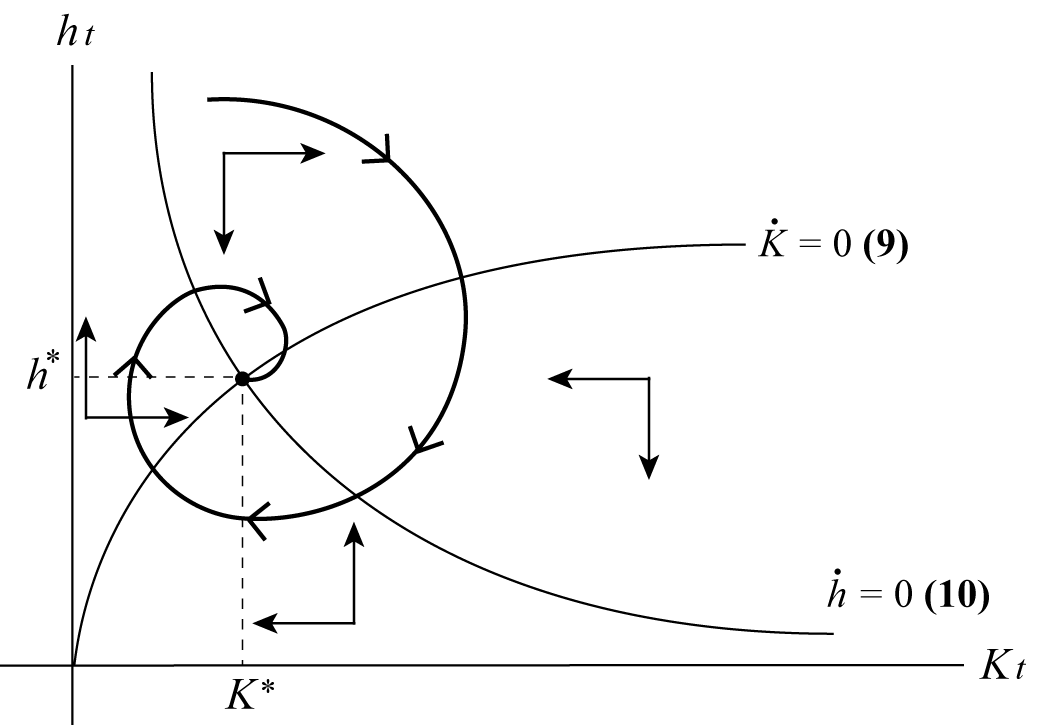
\includegraphics[width=7.8cm]{figure1_ex.png}
  \caption{Phase diagram in $0<\alpha<1$}
  \label{Figure1}
\end{figurehere}

Intuitively, this oscillation implements the following iteration;

\begin{enumerate}
    \item $K^*$ starts to accumulate by reproduction.
    \item Optimal $K^*$ gradually decreases by the increase of acquisition cost.
    \item $K^*$ finally declines since negative flow surpasses positive flow.
    \item Optimal $K^*$ increases again by the decrease of acquisition cost, and back to 1.
\end{enumerate}

\noindent Therefore, on the assumption of diminishing returns, cultural stock eventually converges to the steady state while repeating boom and recession.

\subsection*{Case2: \mbox{\boldmath$1<\alpha$}}
On the other hand, in the case of increasing returns to existing cultural stock, our model takes the dynamics with saddle-path stability shown in figure 2\footnote{We can verify the slope of each loci in the neighbor of the steady-state by log-linearization.
If we set $\hat{h_{t}} = (h_{t}-h^*)/h^*$ and $\hat{K_{t}} = (K_{t}-K^*)/K^*$, equation (9) and (10) can be linearized as $\hat{h_{t}} = (1-\alpha)\hat{K_{t}}$ and $\hat{h_{t}} = -\alpha\hat{K_{t}}$, respectively. Thus, (10) has the steeper slope in the case $1 < \alpha$.}.
Hence, under this case, there is a slight possibility for the steady-state to be unstable\footnote{In addition, we shall find that unstable regions are getting smaller as $\alpha$ increases by the ratio between the slopes of both linearized loci: $\lim_{\alpha \to \infty}{(1-\alpha)}/{-\alpha} = 1$}.\vspace{0.2in}

\begin{figurehere}
  \centering
  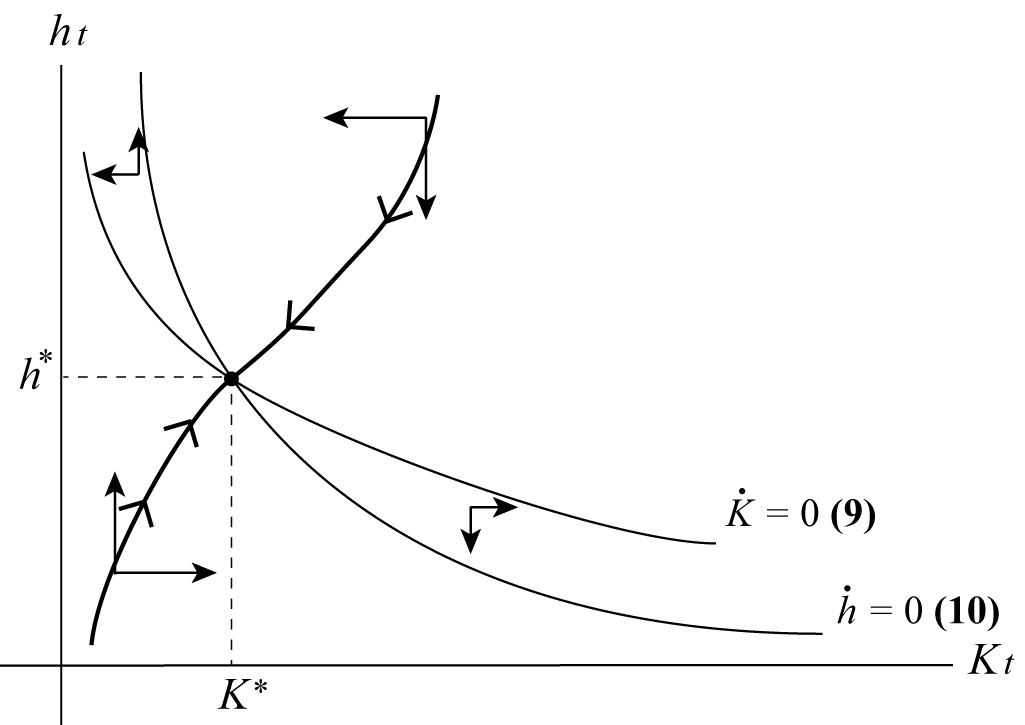
\includegraphics[width=7.8cm]{figure2_ex.png}
  \caption{Phase diagram in $1<\alpha$}
  \label{Figure2}
\end{figurehere}

\subsection*{Case3: \mbox{\boldmath$-1<\alpha<0$}}
Then, if we let cultural reproduction be a decreasing function of existing cultural stock
and $\alpha$ be $-1<\alpha<0$, transitional dynamics follows the stable paths depicted in figure 3.
Thus, the steady-state is stable regardless of initial values.\vspace{0.2in}

\begin{figurehere}
  \centering
  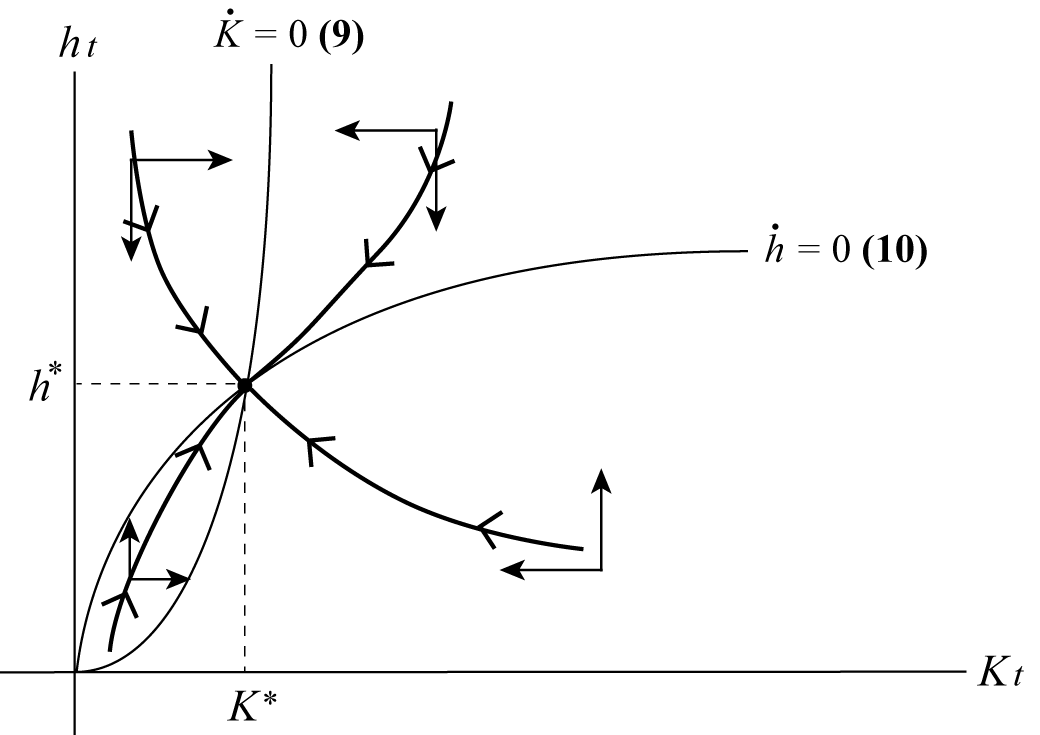
\includegraphics[width=7.8cm]{figure3_ex.png}
  \caption{Phase diagram in $-1<\alpha<0$}
  \label{Figure3}
\end{figurehere}

\begin{table*}[tb]
    \centering
    \caption{Growth paths and their stability}
    \begin{tabular}{lcccc}
        \hline
        &$\alpha<-1$&$-1<\alpha<0$&$0<\alpha<1$&$1<\alpha$\\
        \hline
        Path&stable&stable&stable&saddle\\
        Stability&stable&stable&stable&almost stable\\
        \hline
    \end{tabular}
\label{table:name}
\end{table*}

\subsection*{Case4: \mbox{\boldmath$\alpha<-1$}}
Finally, even if $\alpha$ is less than negative one, stability is the same with Case 3
though equation (10) switches to convex as represented in figure 4.\vspace{0.2in}

\begin{figurehere}
  \centering
  
\includegraphics[width=7.8cm]{figure4_ex.png}
  \caption{Phase diagram in $\alpha<-1$}
  \label{Figure4}
\end{figurehere}

Table 1 summarizes all results derived above.
Although each transitional dynamic takes a different path, they are all stable except a certain situation in Case 2.
Therefore, we conclude that the steady-state is almost stable.

\section{Conclusion}

As a result of the dynamic analysis, the following two main conclusions were obtained:

\begin{itemize}
    \item The steady-state value of cultural stock is not affected by its quality and evaluation.
    \item The steady-state is stable except a certain case with increasing returns.
\end{itemize}

Hence, quality and evaluation are actually neutral to the amount of cultural stock which finally accumulates.
This implies, practically, that indirect policies would be more effective to cultural stock by supporting an environment where individuals can easily utilize well-archived culture and thereby exert their creativity, rather than direct policies which interfere in the quality and evaluation of contents themselves.
We could consider digital archiving as an example of the former, and awarding or certification system as that of the latter.

This research predicts some elemental dynamics of cumulative culture resulting from rationality and expectation and suggests some essentially effective factors to the amount of cultural stock in the long run.
Further improvements can be considered in both theoretical and empirical fields.
Needless to say, theoretical extensions would make our model more realistic by loosening the aforementioned strong simplifications: homogeneous culture, no-human capital and no-uncertainty, and empirical data would also make our model more persuasive by supporting the existence of concrete cultural traits suitable for proposed dynamics.
Despite those limitations, however, our model could work as a benchmark in tackling more complex issues on cumulative culture since its structure and implications are sufficiently generalized and robust.

\section*{Appendix}

\hypertarget{appa}{
\subsection*{Derivation of the Euler Equation}
}
For optimization, the Hamiltonian must satisfy the following first-order conditions,
\begin{align} % FOC
    \frac{\partial J}{\partial h_t}  & =
    e^{-\rho t}\frac{\partial u_1}{\partial M_t}\frac{\partial M_t}{\partial h_t} + v_t \frac{\partial M_t}{\partial h_t} = 0 \tag{A-1} \\
    \frac{\partial J}{\partial K_t}  & =
    e^{-\rho t}\left(\frac{\partial u_1}{\partial M_t}\frac{\partial M_t}{\partial K_t} - \frac{\partial u_2}{\partial K_t} \right) + v_t \left(\frac{\partial M_t}{\partial K_t} - \delta\right) = -\dot{v} \tag{A-2}
\end{align}

\noindent Derivatives associated with objective function can be both obtained from (3).
\begin{align}
    \frac{\partial u_1}{\partial M_t} & =  M_{t}^{-\frac{1}{\sigma}} \tag{A-3} \\
    \frac{\partial u_2}{\partial K_t} & =  \eta \tag{A-4}
\end{align}

\noindent By using (A-3), (A-1) is simplified as follows.
\begin{align}
    e^{-\rho t}M_{t}^{-\frac{1}{\sigma}} = -v_t \tag{A-5}
\end{align}

\noindent Then, taking logarithms and time derivatives of (A-5) leads to the negative growth rate of costate variable.
\begin{align}
    \rho + \frac{1}{\sigma}\frac{\dot M}{M} = - \frac{\dot v}{v} \tag{A-6}
\end{align}

\noindent In terms of (A-2), the same rate can also be derived by dividing both sides by $v$ and substituting (A-3), (A-4) and (A-5).
\begin{align}
    \eta M_{t}^{-\frac{1}{\sigma}} - \delta =  -\frac{\dot v}{v} \tag{A-7}
\end{align}

\noindent Finally, we obtain the Euler equation as (8) from (A-6) and (A-7).

\subsection*{Optimal intellectual property rights}
Our model has an additional implication for intellectual property rights if we assume their excludability increases both creativity and acquisition cost per a unit of culture\footnote{Note that this analysis is just from the viewpoint of social planner. The one who gets more incentive and the one who owes additional acquisition cost would be different in reality.}.
We shall find it convenient here to set ${\sigma}^{-1}$ as $\theta$ and $\theta$ decreases as the excludability gets strong
(That is, curvature of $u_{1}$ approaches linear).
Thus, if we focus on $K^*$, it shifts to
\begin{align}
    K^*_{ip} = \left(\frac{\rho + \delta}{\eta + \eta_{ip}}\right)^{\frac{1}{\theta - \theta_{ip}}}\frac{1}{\delta} \tag{A-8}
\end{align}

\noindent where $K^*_{ip}$ is the steady-state amount of cultural stock with intellectual property rights.
Accordingly, $K^* < K^*_{ip}$ requires the following condition.
\begin{align}
    \left(\frac{\rho + \delta}{\eta}\right)^{\frac{1}{\theta}} < \left(\frac{\rho + \delta}{\eta + \eta_{ip}}\right)^{\frac{1}{\theta - \theta_{ip}}} \tag{A-9}
\end{align}

\noindent By rearranging and taking logarithms, approximately we get,
\begin{align}
    \frac{\eta_{ip}/\eta}{\theta_{ip}/\theta} < \ln{\left(\frac{\rho + \delta}{\eta}\right)} \tag{A-10}
\end{align}

\noindent (A-10) is the condition for intellectual property rights to be effective in the long run, where
$\theta_{ip}/\theta$ is the increasing rate of creativity and $\eta_{ip}/\eta$ is that of acquisition cost; each denotes positive and negative contribution\footnote{If we adhere to using $\sigma$, (A-9) becomes $\frac{\eta_{ip}/\eta}{(\sigma+\sigma_{ip})/\sigma_{ip}} < \ln{\left(\frac{\rho + \delta}{\eta}\right)}$.}.
Therefore, we can say that the rights are useful only if positive per negative contribution is less than the composition of exogenous parameters: $\ln{\left(\frac{\rho + \delta}{\eta}\right)}$.


\begin{thebibliography}{1}
\makeatletter
\def\@biblabel#1{}
\let\old@bibitem\bibitem
\def\bibitem#1{\old@bibitem{#1}\leavevmode\kern-\bibindent}
\makeatother

  \hypertarget{boyd}{\bibitem{boyd} Boyd, R., and P. J. Richerson. (1985).
    ``Culture and the evolutionary process,''  Chicago: University of Chicago Press.
    pp.147-151, Manchester, U.K., Aug. 1988.}
  \hypertarget{csik}{\bibitem{csik} Csikszentmihalyi, M. (2014).
    ``The systems model of creativity and its applications. In D. K. Simonton (Ed.),'' The Wiley Handbook of Genius (no.17525-17862). Wiley-Blackwell. (Kindle edition).}
  \hypertarget{henrich}{\bibitem{henrich} Henrich, J. (2004).
    ``Demography and cultural evolution: How adaptive cultural processes can produce maladaptive losses—The Tas- manian case.'' American Antiquity, 69(2), 197–214.}
  \hypertarget{lehman}{\bibitem{lehman} Lehmann, L., Wakano, J. Y., Aoki, K. (2013).
    ``On optimal learning schedules and the marginal value of cumulative cultural evolution.'' Evolution. 2013 May; 67(5):1435-45. doi: 10.1111/evo.12040. Epub 2013 Jan 23.}
  \hypertarget{mesoa}{\bibitem{mesoa} Mesoudi, A. (2011a).
    ``Variable cultural acquisition costs constrain cumulative cultural evolution.'' PLos One, 6, e18239. doi:10.1371/journal.-pone.0018239.}
  \hypertarget{mesob}{\bibitem{mesob} Mesoudi, A. (2011b).
    ``Cultural evolution: how darwinian theory can explain human culture and synthesize the social sciences,'' Chicago and London: University of Chicago Press.}
  \hypertarget{romer}{\bibitem{romer} Romer, D. (2011).
    ``Advanced Macroeconomics,'' 4th ed. New York: McGraw-Hill Education.}
\end{thebibliography}

{\small \theendnotes}

\end{document}
